\section{What I did}
\subsection{Dataset}
The dataset used for this project is a mixed dataset from multiple sources, Mathhub and the Learner model.
The course materials and the knowledge graph built from them are available on Mathhub. Every symbol on Mathhub has a URL and a content of it. 
The Leaner model has the understanding level of every symbol in Mathhub in six dimensions. 

\usetikzlibrary {calc,positioning,shapes.misc}
\tikzset{terminal/.style={rectangle,draw,inner sep=2pt}}
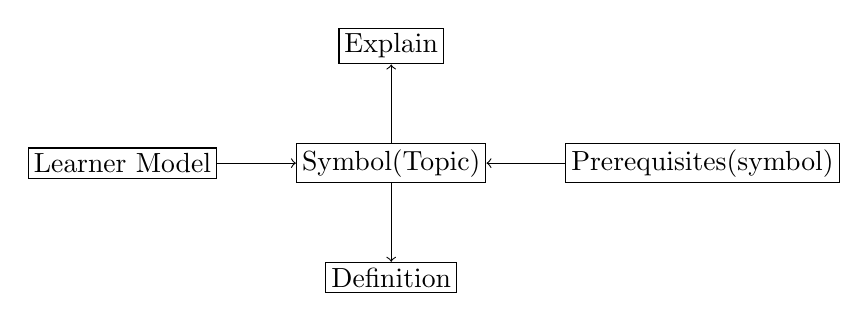
\begin{tikzpicture}
  \node (leaner)   [terminal]                        {Learner Model};
  \node (symbols) [terminal,right=of leaner]           {Symbol(Topic)};
  \node (prerequestest)     [terminal,right=of symbols]         {Prerequisites(symbol)};
  \node (explian) [terminal, above=of symbols] {Explain};
  \node (definition) [terminal, below=of symbols] {Definition};

  \path (leaner)   edge[->]           (symbols)  % simple edges
        (prerequestest) edge[->]           (symbols)
        (symbols) edge[->] (explian)
        (symbols) edge[->] (definition);
        
\end{tikzpicture}


